\documentclass[11pt]{article}

\usepackage[margin=1in, paperwidth=8.5in, paperheight=11in]{geometry}
\usepackage{amsfonts}
\usepackage{graphicx}

\def\eq1{y=\frac{x}{3x^2+x+1}}

\begin{document}
\title{practice \LaTeX \ session}
\author{Mani Nandadeep Medicharla}
\date{\today}
\maketitle

The set of natural numbers is denoted by $\mathbb{N}$

The set of integers are denoted by $\mathbb{Z}$

The set of Real are denoted by $\mathbb{R}$

Graph $\eq1$

identify the asymptotes for the graph of $\eq1$

\begin{center}
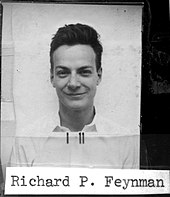
\includegraphics[width=5cm]{img.jpg}
\end{center}

\begin{center}
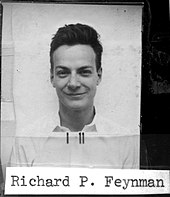
\includegraphics[scale=0.5]{img.jpg}
\end{center}

\begin{center}
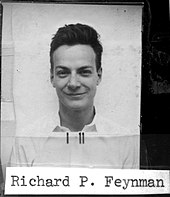
\includegraphics[angle=45]{img.jpg}
\end{center}

\end{document}